\documentclass[a4paper,11pt]{article}
\usepackage[utf8]{inputenc}
\usepackage{amsmath}
\usepackage{amsfonts}
\usepackage{amssymb}
\usepackage{graphicx}
\usepackage{braket}

\numberwithin{equation}{section}
\renewcommand\thesubsection{\alph{subsection}}
\newcommand{\bvp}[1]{\mathbf{#1}'}
\newcommand{\bv}[1]{\mathbf{#1}}


%opening
\title{Statmech II HW4}
\author{Vince Baker}

\begin{document}

\maketitle

\section{Problem 6.2}
We derive the expressions for $\braket{n_e^2}-\braket{n_e}^2$ starting from the probabilities.
\\ \\
For Bose-Einstein statistics:
\begin{align}
 \braket{n_e^2} &= \sum_n^\infty n^2 \rho_e (n)\\
 \braket{n_e^2} &= \sum_n^\infty n^2 \frac{\braket{n_e}^n}{(\braket{n_e}+1)^{n+1}}\\
\end{align}
We use the relation $\sum_n^\infty n^2x^n = \frac{x(x+1)}{(1-x)^3}$ and pull out a factor of $1/(\braket{n_e}+1)$.
\begin{align}
 \braket{n_e^2} &= \frac{1}{\braket{n_e}+1}\left(\frac{\frac{\braket{n_e}}{\braket{n_e}+1}(1+\frac{\braket{n_e}}{\braket{n_e}+1})}
		  {(1-\frac{\braket{n_e}}{\braket{n_e}+1})^3} \right)\\
 \braket{n_e^2} &= \frac{\braket{n_e}}{(\braket{n_e+1})^2}
		    \frac{2\braket{n_e}+1}{\braket{n_e}+1}\left(\braket{n_e}+1\right)^3\\
 \braket{n_e^2} &= 2\braket{n_e}^2+\braket{n_e}\\
 \sigma^2 &= \braket{n_e}^2+\braket{n_e}
\end{align}
We also prove the differential relation:
\begin{align}
 kT \frac{\partial \braket{n_e}}{\partial \mu} &= kT \frac{\partial}{\partial \mu}\left(\frac{1}{z^{-1}e^{\beta e}-1} \right)\\
 kT \frac{\partial \braket{n_e}}{\partial \mu} &= \left( \frac{1}{(z^{-1}e^{\beta e}-1)^2} + \frac{1}{z^{-1}e^{\beta e}-1}\right)\\
 kT \frac{\partial \braket{n_e}}{\partial \mu} &= \braket{n_e}^2+\braket{n_e} = \sigma^2
\end{align}
\\ \\
For Fermi-Dirac statistics:
\begin{align}
  \rho_e(n) &= \left(1-\braket{n_e},\braket{n_e} \right)\\ 
 \braket{n_e^2} &= \frac{0^2*(1-\braket{n_e})}{1}+\frac{1^2*\braket{n_e}}{1} = \braket{n_e}\\
 \sigma^2 &=\braket{n_e}-\braket{n_e}^2
\end{align}
We also prove the differential relation:
\begin{align}
 kT \frac{\partial \braket{n_e}}{\partial \mu} &= kT \frac{\partial}{\partial \mu}\left(\frac{1}{z^{-1}e^{\beta e}+1} \right)\\
 kT \frac{\partial \braket{n_e}}{\partial \mu} &= \left(\frac{1}{z^{-1}e^{\beta e}+1}-\frac{1}{(z^{-1}e^{\beta e}+1)^2} \right)\\
 kT \frac{\partial \braket{n_e}}{\partial \mu} &= \braket{n_e}-\braket{n_e}^2 = \sigma^2
\end{align}
\\ \\
For Maxwell-Boltzmann statistics:
\begin{align}
 \braket{n_e^2} &= \sum n^2\frac{\braket{n_e}^n}{n!}e^{-\braket{n_e}}\\
 \braket{n_e^2} &= e^{-\braket{n_e}}\sum (n-1+1)\frac{\braket{n_e}^n}{(n-1)!}\\
 \braket{n_e^2} &= e^{-\braket{n_e}}\left( \sum \frac{\braket{n_e}^n}{(n-2)!} +
                                             \sum \frac{\braket{n_e}^n}{(n-1)!}\right)\\
 \braket{n_e^2} &= e^{-\braket{n_e}}\left( \braket{n_e}^2e^{\braket{n_e}}+\braket{n_e} e^{\braket{n_e}} \right)\\
 \braket{n_e^2} &= \braket{n_e}^2+\braket{n_e}\\
 \sigma^2 &= \braket{n_e}
\end{align}
We also prove the differential relation:
\begin{align}
 \sigma^2 &= \braket{n_e}\\
 kT \frac{\partial \braket{n_e}}{\partial \mu} &= kT \frac{\partial}{\partial \mu}\left(ze^{-\beta e} \right)\\
 kT \frac{\partial \braket{n_e}}{\partial \mu} &= \braket{n_e}
\end{align}
\\
\section{Problem 6.3}
If the possible numer of particles in a level $n_e$ is restricted to values $\le \ell$, then we can write the grand partition function:
\begin{align}
 Z &= \prod_e \sum_{n_e=0}^\ell (ze^{-\beta e})^{n_e}
\end{align}
Using the expression for the first $\ell$ terms of a power series we can write this:
\begin{align}
 Z &= \prod_e \left( \frac{1-(ze^{-\beta e})^{\ell+1}}{1-ze^{-\beta e}} \right)\\
 \Omega &= \ln{Z} = \sum_e \ln{\left( \frac{1-(ze^{-\beta e})^{\ell+1}}{1-ze^{-\beta e}} \right)}\\
 \braket{n_e} &= -\frac{1}{\beta}\left(\frac{\partial \Omega}{e} \right)\\
 \braket{n_e} &= -\frac{1}{\beta}\left( \frac{1}{1+(ze^{-\beta e})^{\ell+1}}\beta(\ell+1)(ze^{-\beta e})^{\ell+1} 
		  -\frac{1}{1-ze^{-\beta e}}\beta ze^{-\beta e}\right)\\
 \braket{n_e} &= \frac{ze^{-\beta e}}{1-ze^{-\beta e}}
		  -\frac{(\ell+1)(ze^{-\beta e})^{\ell+1}}{1-(ze^{-\beta e})^{\ell+1}}\\
 \braket{n_e} &= \frac{1}{z^{-1}e^{\beta e}-1}
		  -\frac{\ell+1}{(z^{-1}e^{\beta e})^{\ell+1}-1}\\
\end{align}
\\
For Fermi-Dirac statistics $\ell=1$, and we recover the expected result:
\begin{align}
 \braket{n_e} &= \frac{1}{z^{-1}e^{\beta e}-1}
		  -\frac{2}{(z^{-1}e^{\beta e})^2-1}\\
 u &\equiv z^{-1}e^{\beta e}\\
 \frac{1}{u-1}-\frac{2}{(u-1)(u+1)} &= \frac{u-1}{(u-1)(u+1)} = \frac{1}{u+1}\\
 \braket{n_e} &= \frac{1}{z^{-1}e^{\beta e}+1}
\end{align}
\\
For Bose-Einstein statistics $\ell=\infty$. 
The right-hand term goes to 0, so we are left with $\braket{n_e} = \frac{1}{z^{-1}e^{\beta e}-1} $ as expected.
\section{Problem 9.5}
a) We calculate the parametric equation of state for the grand parition function $Z=(1+z)^V(1+z^{\alpha V}) $:
\begin{align}
 \frac{P}{kT} &= V^{-1}\ln{Z}\\
 \frac{P}{kT} &= \ln{(1+z)}+\frac{1}{V}\ln{(1+z^{\alpha V})}\\
 \frac{1}{v}  &= V^{-1}z\frac{\partial}{\partial z}\ln{Z}\\
 \frac{1}{v}  &= \left(\frac{z}{1+z}+\frac{\alpha}{z^{-\alpha V}+1} \right)
\end{align}
The graphs below show the discontinuities at $z=1$ and the resulting first-order phase transition.
\\
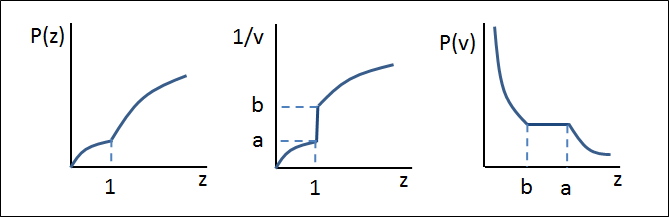
\includegraphics{statmech_p9_5}
\\ 
For $z<1$ as $V \rightarrow \infty$ we have $\frac{1}{v}=\frac{z}{1+z}$.\\
For $z>1$ as $V \rightarrow \infty$ we have $\frac{1}{v}=\frac{z}{1+z}+\alpha$.
\\ \\
b) For fixed V the roots in the complex plane for $Re(z)>0$ are $z=(-1)^{\pm\frac{1}{\alpha V}} $.
As $V \rightarrow \infty$ the roots converge to $z=1+i0$.
\\ \\
c) In the ``gas'' phase $z>1$  the equation of state as $V \rightarrow \infty$ is:
\begin{align}
 \frac{P}{kT} &= \ln{(1+z)}+\alpha \ln{z}\\
 \frac{1}{v}  &= \frac{z}{z+1}+\alpha
\end{align}
Where in 3.6 we have taken the limit $V \rightarrow \infty$ before taking the derivative.
These equations are continuous across $z=1$ and so do not exhibit a phase transition.

\end{document}
